\documentclass[journal]{IEEEtran}

% *** CITATION PACKAGES ***
\usepackage{cite}

% *** GRAPHICS RELATED PACKAGES ***
%
\ifCLASSINFOpdf
\usepackage[pdftex]{graphicx}
  % declare the path(s) where your graphic files are
  % \graphicspath{{../pdf/}{../jpeg/}}
  % and their extensions so you won't have to specify these with
  % every instance of \includegraphics
  % \DeclareGraphicsExtensions{.pdf,.jpeg,.png}
\else
  % or other class option (dvipsone, dvipdf, if not using dvips). graphicx
  % will default to the driver specified in the system graphics.cfg if no
  % driver is specified.
  % \usepackage[dvips]{graphicx}
  % declare the path(s) where your graphic files are
  % \graphicspath{{../eps/}}
  % and their extensions so you won't have to specify these with
  % every instance of \includegraphics
  % \DeclareGraphicsExtensions{.eps}
\fi
% graphicx was written by David Carlisle and Sebastian Rahtz. It is
% required if you want graphics, photos, etc. graphicx.sty is already
% installed on most LaTeX systems. The latest version and documentation
% can be obtained at: 
% http://www.ctan.org/pkg/graphicx
% Another good source of documentation is "Using Imported Graphics in
% LaTeX2e" by Keith Reckdahl which can be found at:
% http://www.ctan.org/pkg/epslatex
%
% latex, and pdflatex in dvi mode, support graphics in encapsulated
% postscript (.eps) format. pdflatex in pdf mode supports graphics
% in .pdf, .jpeg, .png and .mps (metapost) formats. Users should ensure
% that all non-photo figures use a vector format (.eps, .pdf, .mps) and
% not a bitmapped formats (.jpeg, .png). The IEEE frowns on bitmapped formats
% which can result in "jaggedy"/blurry rendering of lines and letters as
% well as large increases in file sizes.
%
% You can find documentation about the pdfTeX application at:
% http://www.tug.org/applications/pdftex






% *** PDF, URL AND HYPERLINK PACKAGES ***
%
%\usepackage{url}
% url.sty was written by Donald Arseneau. It provides better support for
% handling and breaking URLs. url.sty is already installed on most LaTeX
% systems. The latest version and documentation can be obtained at:
% http://www.ctan.org/pkg/url
% Basically, \url{my_url_here}.


% correct bad hyphenation here
\hyphenation{op-tical net-works semi-conduc-tor}


\begin{document}
%
% paper title
% Titles are generally capitalized except for words such as a, an, and, as,
% at, but, by, for, in, nor, of, on, or, the, to and up, which are usually
% not capitalized unless they are the first or last word of the title.
% Linebreaks \\ can be used within to get better formatting as desired.
% Do not put math or special symbols in the title.
\title{Segmentación de Glóbulos Rojos en Imágenes Digitales Usando OpenCV}


\author{Álvaro Salgado López}

% note the % following the last \IEEEmembership and also \thanks - 
% these prevent an unwanted space from occurring between the last author name
% and the end of the author line. i.e., if you had this:
% 
% \author{....lastname \thanks{...} \thanks{...} }
%                     ^------------^------------^----Do not want these spaces!
%
% a space would be appended to the last name and could cause every name on that
% line to be shifted left slightly. This is one of those "LaTeX things". For
% instance, "\textbf{A} \textbf{B}" will typeset as "A B" not "AB". To get
% "AB" then you have to do: "\textbf{A}\textbf{B}"
% \thanks is no different in this regard, so shield the last } of each \thanks
% that ends a line with a % and do not let a space in before the next \thanks.
% Spaces after \IEEEmembership other than the last one are OK (and needed) as
% you are supposed to have spaces between the names. For what it is worth,
% this is a minor point as most people would not even notice if the said evil
% space somehow managed to creep in.








% If you want to put a publisher's ID mark on the page you can do it like
% this:
%\IEEEpubid{0000--0000/00\$00.00~\copyright~2015 IEEE}
% Remember, if you use this you must call \IEEEpubidadjcol in the second
% column for its text to clear the IEEEpubid mark.



% use for special paper notices
%\IEEEspecialpapernotice{(Invited Paper)}


\markboth{Procesamiento Y Clasificación de Datos, 13 Febrero 2025}{}

% make the title area
\maketitle



%\IEEEpeerreviewmaketitle



\section{Introducción}
% The very first letter is a 2 line initial drop letter followed
% by the rest of the first word in caps.
% 
% form to use if the first word consists of a single letter:
% \IEEEPARstart{A}{demo} file is ....
% 
% form to use if you need the single drop letter followed by
% normal text (unknown if ever used by the IEEE):
% \IEEEPARstart{A}{}demo file is ....
% 
% Some journals put the first two words in caps:
% \IEEEPARstart{T}{his demo} file is ....
% 
% Here we have the typical use of a "T" for an initial drop letter
% and "HIS" in caps to complete the first word.
\IEEEPARstart
{L}{a} segmentación de imágenes es una técnica clave en el análisis de imágenes biomédicas, permitiendo identificar y aislar elementos de interés dentro de una muestra visual. En este proyecto, se implementan técnicas de procesamiento de imágenes para la segmentación de glóbulos rojos, utilizando la biblioteca OpenCV. El objetivo principal es extraer de manera precisa los glóbulos rojos presentes en imágenes, aplicando umbrales adaptativos y operaciones morfológicas que optimizan la detección y separación de estos elementos.

La identificación precisa de glóbulos rojos tiene aplicaciones fundamentales en el diagnóstico de enfermedades, como anemia, leucemia y otras patologías relacionadas con la sangre. En este contexto, las herramientas computacionales como OpenCV permiten desarrollar soluciones eficientes y reproducibles para el análisis automatizado de imágenes biomédicas.
% You must have at least 2 lines in the paragraph with the drop letter
% (should never be an issue)

\section{Metodología}
El proceso de segmentación de glóbulos rojos se llevó a cabo aplicando técnicas básicas de procesamiento de imágenes digitales mediante la biblioteca OpenCV. A continuación, se describen los pasos realizados:
\subsection{Conversión a Escala de Grises}
La imagen original fue convertida a escala de grises, este paso permitió simplificar la representación de la imagen, enfocándose únicamente en la intensidad de los píxeles.
\subsection{Suavizado de la Imagen}
Para reducir el ruido y mejorar la precisión en las etapas posteriores, se aplicó un filtro de mediana con un kernel de tamaño 5. Esto ayudó a eliminar pequeñas variaciones no deseadas en la imagen.
\subsection{Aplicación de Umbral Adaptativo}
Se utilizó un umbral adaptativo basado en el método Gaussiano para segmentar los glóbulos rojos. Este método ajusta dinámicamente el umbral en función de las condiciones locales de la imagen, permitiendo binarizar de manera robusta las regiones de interés.
\subsection{Coloración de la Segmentación}
La imagen binarizada resultante fue convertida a una imagen a color. Posteriormente, se asignó un color verde a las regiones segmentadas correspondientes a los glóbulos rojos.
\subsection{Superposición de Imágenes}
Para validar visualmente los resultados, se generó una imagen combinada, en la cual la imagen segmentada se superpuso sobre la imagen original con un nivel de transparencia ajustado (alpha = 0.5). Este paso permitió observar claramente las regiones segmentadas en su contexto original.

\section{Resultados}
En la Figura \ref{globulos}, se ilustran los resultados obtenidos tras aplicar el proceso de segmentación de glóbulos rojos. La imagen de la izquierda corresponde a la representación original en formato RGB, donde se pueden observar las características iniciales de la muestra, como el contraste y la disposición de los glóbulos rojos.

\begin{figure}
    \centering
    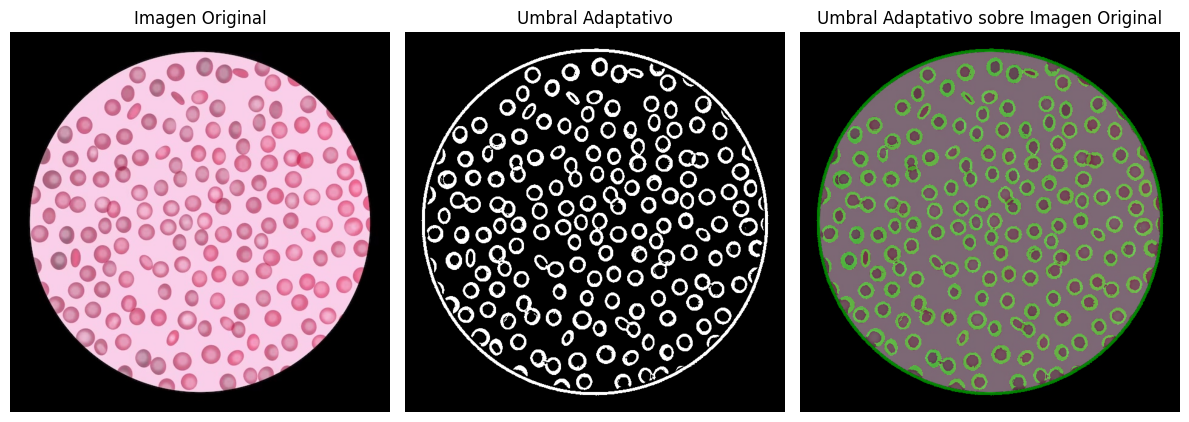
\includegraphics[width=0.9\linewidth]{Figs/Globulos.png}
    \caption{Resultados del proceso de segmentación de glóbulos rojos}
    \label{globulos}
\end{figure}
En el centro, se muestra el resultado del umbral adaptativo aplicado a la imagen suavizada. Este procesamiento resalta las regiones correspondientes a los glóbulos rojos en blanco, mientras que el fondo y otras áreas irrelevantes permanecen en negro. La binarización lograda permite una identificación clara y precisa de las estructuras de interés.

Finalmente, la imagen combinada, ubicada a la derecha, muestra la segmentación superpuesta sobre la imagen original. Las áreas segmentadas están destacadas en color verde, lo que facilita la validación visual de los resultados en el contexto original. Esta representación demuestra la efectividad del proceso y permite corroborar que las regiones segmentadas corresponden a los glóbulos rojos presentes en la muestra.

\section{Conclusión}
El proceso de segmentación de glóbulos rojos utilizando técnicas de umbral adaptativo ha demostrado ser eficaz en la identificación y aislamiento de estas estructuras en imágenes biomédicas. La aplicación de un umbral adaptativo permitió obtener una binarización robusta, incluso ante variaciones en la iluminación de la imagen. La superposición de la segmentación sobre la imagen original proporcionó una validación visual clara, evidenciando que las regiones segmentadas corresponden a los glóbulos rojos presentes en la muestra.

Este enfoque puede ser útil en la automatización de procesos de análisis de imágenes médicas, como la identificación de patologías sanguíneas, y podría mejorarse aún más mediante el uso de técnicas avanzadas de procesamiento o integración con métodos de aprendizaje automático para optimizar la precisión en contextos más complejos.

% Can use something like this to put references on a page
% by themselves when using endfloat and the captionsoff option.
\ifCLASSOPTIONcaptionsoff
  \newpage
\fi



% trigger a \newpage just before the given reference
% number - used to balance the columns on the last page
% adjust value as needed - may need to be readjusted if
% the document is modified later
%\IEEEtriggeratref{8}
% The "triggered" command can be changed if desired:
%\IEEEtriggercmd{\enlargethispage{-5in}}

% references section

% can use a bibliography generated by BibTeX as a .bbl file
% BibTeX documentation can be easily obtained at:
% http://mirror.ctan.org/biblio/bibtex/contrib/doc/
% The IEEEtran BibTeX style support page is at:
% http://www.michaelshell.org/tex/ieeetran/bibtex/
%\bibliographystyle{IEEEtran}
% argument is your BibTeX string definitions and bibliography database(s)
%\bibliography{IEEEabrv,../bib/paper}
%
% <OR> manually copy in the resultant .bbl file
% set second argument of \begin to the number of references
% (used to reserve space for the reference number labels box)

%\bibliographystyle{IEEEtran} % Estilo de citas de IEEE
%\bibliography{referencias} % Nombre de tu archivo .bib


\end{document}


